\subsection{Treatment of topography in child domain} \label{subsec:nest_topo}
%------------------------------------------------------
In the nesting experiment, the resolutions of the topography were different between the parent and the child domains due to their different spatial resolutions. In the relaxation area of the child domain (refer to Section \ref{subsec:buffer}), the atmospheric variables were nudged toward those of the parent domain. If the representations of the topography are different between two domains, the reference data for nudging, calculated in the parent domain, often does not exist. In this case, atmospheric data at the missing levels are estimated by extrapolation. However, this may incur error if the estimation by the extrapolation is not accurate.

In order to avoid such inconsistency due to differences in topographies, the use of ``the topography-copy'' function in \scalerm is recommended. This function copies the topography of the parent domain onto that of the child domain in the relaxation area. If this function is used, the topography of the relaxation area in the child domain perfectly corresponds to that in the parent domain, as shown in \ref{fig_topocopy}.  Furthermore, in order to increase the resolution of topography gradually from that in the parent domain to that in the inner domain, the topography transition area is present on the inside of the relaxation area. In the topography transition area, topography is generated by weighing those of the parent and the child domains. By default, the width of the topography transition area is identical to that of the relaxation area. In the calculation area inside the topography transition area, the topography is given by that of the child domain. If ``the making tool for the complete settings of the experiment'' is used ( refer to \ref{sec:basic_makeconf} ), the topography-copy function is automatically applied.

The file \verb|pp.d0*.conf| mentioned in this section can be generated by  ``the making tool for the complete settings of the experiment'' by renaming \\ \verb|${Tutorial_dir}/real/sample/USER.online-nesting.sh| as \verb|USER.sh|. This may help users understand this setting. The configuration and execution methods are explained below.

\begin{figure}[tbh]
\begin{center}
  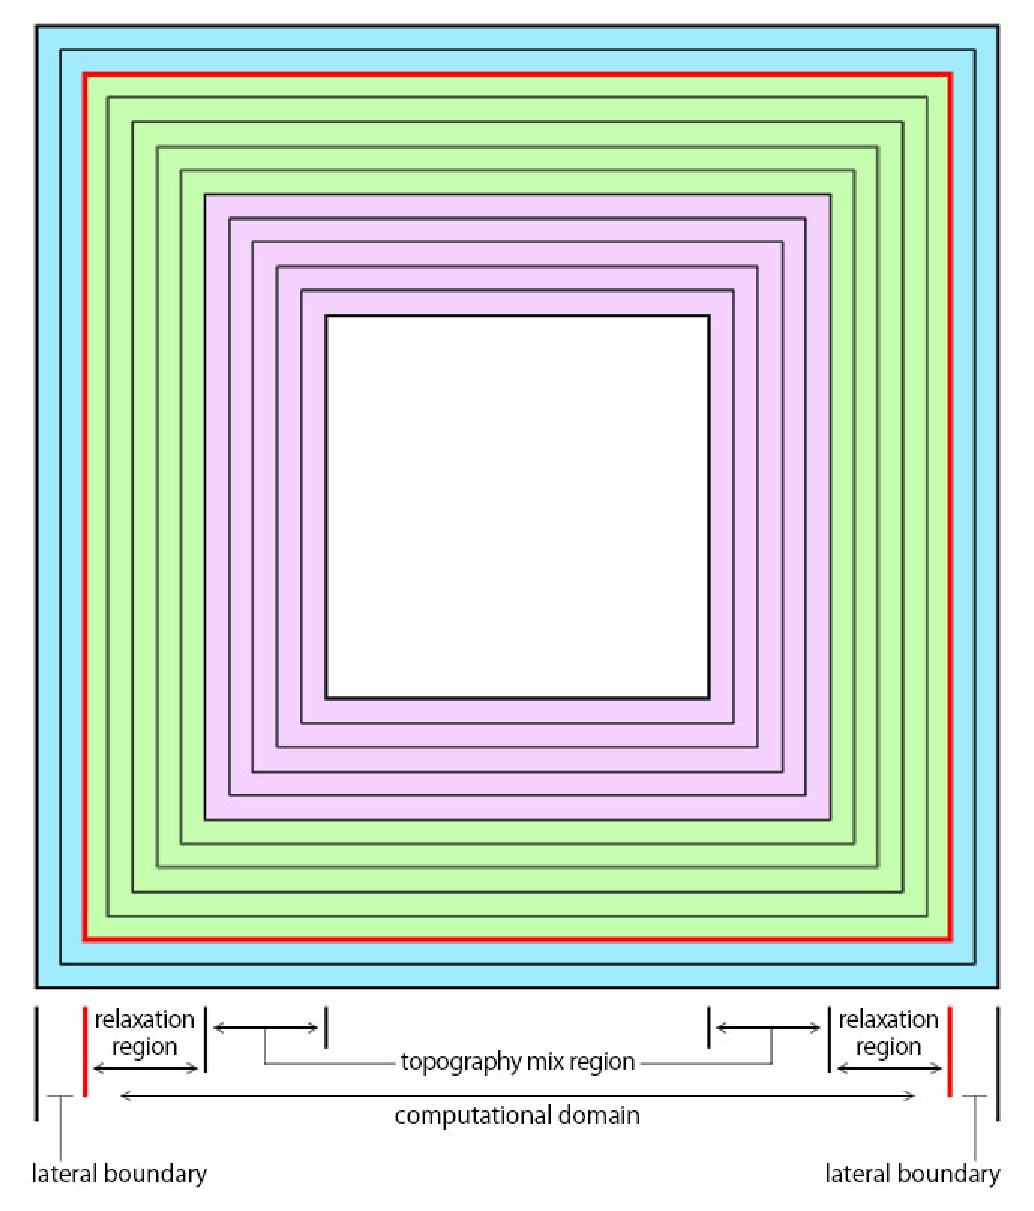
\includegraphics[width=0.4\hsize]{./figure/topo_copy.pdf}\\
  \caption{Horizontal distribution of topography when the topography-copy function is applied.
    The outermost grids shaded in light blue represent the \texttt{HALO} region, and the number of grids depends on
    the horizontal advection scheme.
    These grids are the lateral boundary. The area demarcated by the red line is the calculation domain.
    The green- and rose-colored areas are the relaxation and the topographical transition areas, respectively.
    The innermost area is where the resolution of topography is the same as that of the original child domain.
    In the topography transition area, topography is altered gradually from that of
    the parent domain to the original child domain.
}
  \label{fig_topocopy}
\end{center}
\end{figure}



\subsubsection{How to use topography-copy function}

In order to output a catalog file that gives the size of the parent domain to the child domain when \verb|scale-rm_pp| generates the topography of the parent domain, the following configuration is needed in \verb|pp.d01.conf| :
\editboxtwo{
\verb|&PARAM_DOMAIN_CATALOGUE|  & \\
\verb| DOMAIN_CATALOGUE_FNAME  = "latlon_domain_catalogue.d01.txt",| & Name of catalog file\\
\verb| DOMAIN_CATALOGUE_OUTPUT = .true.,| & Whether catalog file is output \\
\verb|/|  & \\
}
The other parameters are the same as usual.

To use the parent topography for the topography-copy function, edit file \verb|pp.d02.conf| for the child domain as follows.
Here, the output data of topography in the parent domain is assumed to be saved as file \verb|topo_d01.pe***.nc| in SCALE netCDF file format.
As other file formats, GrADS and WRF-ARW formats are supported.
\editboxtwo{
\verb|&PARAM_NEST| & \\
\verb| OFFLINE_PARENT_BASENAME   = "topo_d01", | & base name of the file of the parent domain \\
\verb| OFFLINE_PARENT_PRC_NUM_X  = 2,          | & \verb|PRC_NUM_X| of the parent domain\\
\verb| OFFLINE_PARENT_PRC_NUM_Y  = 2,          | & \verb|PRC_NUM_Y| of the parent domain\\
\verb| LATLON_CATALOGUE_FNAME    = "latlon_domain_catalogue.d01.txt",| & catalog file for the parent domain  \\
\verb|/| &\\
 & \\
\verb|&PARAM_CNVTOPO| & \\
\verb| ~ .... ~     | & \\
\verb| CNVTOPO_copy_parent     = .true.,| & whether the topography-copy function is applied\\
\verb|/             | & \\
 & \\
\verb|&PARAM_COPYTOPO| & \\
\verb| COPYTOPO_IN_BASENAME   = "topo_d01",| & base name of the file of parent topography data \\
\verb| COPYTOPO_IN_FILETYPE   = "SCALE",   | & type of the file of parent topography data (SCALE, GrADS, or WRF-ARW) \\
\verb| COPYTOPO_TRANSITION_DX = -1,        | & Width of transition area in x-direction \\
\verb| COPYTOPO_TRANSITION_DY = -1,        | & Width of transition area in y-direction \\
\verb| COPYTOPO_ENTIRE_REGION = .false.,|    & whether the parent’s topography is copied over the entire child domain\\
\verb| COPYTOPO_LINEAR_H      = .true.,|     & \\
\verb|/| & \\
}
If \nmitem{CNVTOPO_copy_parent} in \namelist{PARAM_CNVTOPO} is \verb|.true.|, the topography-copy function is applied.
\nmitem{COPYTOPO_ENTIRE_REGION} is an option whereby the parent’s topography can be copied over the entire child domain. If this is \verb|.true.|, the topography in the child domain is completely copied from that in the parent domain. \nmitem{COPYTOPO_LINEAR_H} is the parameter to determine which the topography transition method is applied. If \nmitem{COPYTOPO_LINEAR_H} $=$ \verb|.true.|, the ratio of the parent’s topography to the child’s topography is linearly changed. Otherwise, it is changed exponentially.
The width of transition area is specified by \nmitem{COPYTOPO_TRANSITION_DX, COPYTOPO_TRANSITION_DY}. If these have negative value, the default setting is applied: the width of transition area equals to that of relaxation area.

\subsubsection{Generation of topography}
In case of using the topography-copy function, the generation of the topography should start from the parent domain  because a child domain requires the catalog  file of the parent. If the number of domains is greater than three, the order of execution is as follows:
\begin{verbatim}
 $ mpirun -n [number of processes] ./scale-rm_pp pp.d01.conf
 $ mpirun -n [number of processes] ./scale-rm_pp pp.d02.conf
 $ mpirun -n [number of processes] ./scale-rm_pp pp.d03.conf
\end{verbatim}


